\newif\ifmbeformat
\mbeformatfalse

\ifmbeformat
	\documentclass[nogrid]{MBE}%
\else
	\documentclass[twocolumn]{article}
	\usepackage{geometry}
	\newgeometry{
		top=1in,
		bottom=1in,
		outer=1in,
		inner=1in,
	}
	\usepackage{natbib}
	\renewcommand{\baselinestretch}{1.25}		
	\usepackage{authblk}
\fi

\usepackage[normalem]{ulem}
\usepackage{xcolor} 
\newcommand{\revch}[1]{{\color{blue} #1}}
\newcommand{\revcom}[1]{{\color{orange} #1}}
\newcommand{\revrem}[1]{{\color{red} \sout{#1}}}

\usepackage{url}
\usepackage{cuted}
\usepackage{amsmath}
\usepackage{subfig}
%\usepackage{caption}
\usepackage{tabularx}
\usepackage{longtable}
\usepackage{caption}

\usepackage{lipsum}
\usepackage{enumerate}
\usepackage{enumitem}
%load any additional packages
\usepackage{amssymb}
%\usepackage{stackengine}
%\stackMath
\usepackage{amsfonts}
\usepackage{mathtools}
\usepackage{multirow}
\usepackage{bibentry}
%\usepackage{epstopdf} 
%\usepackage{xr}
%\usepackage[landscape,a4paper]{geometry}
\usepackage{booktabs} 
\usepackage{colortbl} 
%\usepackage{xcolor} 
%\usepackage{xfrac}
%\newcommand{ra}[1]{renewcommand{arraystretch}{#1}}
%\usepackage{pdflscape}
%\usepackage{longtable}
%\usepackage{stackrel}
\usepackage{hyperref}
%\usepackage{graphicx}
%\usepackage{svg}
\usepackage{setspace}
%\usepackage{refcheck}
%\usepackage{listings}
%\usepackage{color} 

\usepackage{xr}
\externaldocument[supplementary-]{supplementary}


\newif\iffigures
\figurestrue

\ifmbeformat
\jshort{mst}

\volname{}

\jvolume{0}

\jvol{}

\jissue{0}

\pubyear{2013}

\mstype{Article}

\artid{012}

\access{Advance Access publication March 3, 2013}
\fi

\newcommand{\abstractext}{We present a probabilistic model of protein evolution that captures several important features of protein sequence and structure. The key feature being dependencies between neighbouring amino acid positions that are temporal in nature due to sequence mutations that occur during evolution. The model is trained on a large number of protein alignments and corresponding phylogenetic trees that represent the evolutionary history of the aligned proteins. This yields a model that acts as a rich prior distribution over protein evolution that can be used to perform several important inference tasks. One such task being Bayesian reconstruction of ancestral virus protein sequences, which we demonstrate to have better accuracy than competing methods. The model represents the complete backbone structure of each protein using an angle and bond length representation that realistically captures local features of protein structure. Such local structure evolution is modelled jointly with sequence, permitting ancestral structures to be reconstructed in a phylogenetically rigorous manner. Likewise, the model can perform homology modelling to predict the unknown local backbone structure of a known protein sequence using additional information from potentially large numbers of homologous proteins.  The model is highly flexible with respect to the information that the user can choose to provide, implying that arbitrary combinations of protein sequences and structures can be used when performing various inference tasks. The current model does not capture long-range dependencies that are necessary for accurate homology modelling and reconstruction of ancestral three-dimensional structures. However, it is ultimately expected to be combined with state-of-the-art machine-learning models of protein structure that account for these long-range structural dependencies, but that do not account for evolutionary information that can strongly inform predictions.}

\begin{document}

\title{Reconstructing ancestral protein	sequences and structures}

\ifmbeformat
\author[Golden et al.]{Michael \surname{Golden},$^{\ast,1}$, Jotun Hein,$^{2}$ Thomas Hamerlyck,$^{3}$ and Oliver Pybus,$^{1}$}

\address{
$^{1}$Department of Zoology, University of Oxford, UK\\
$^{2}$Department of Statistics, University of Oxford, UK\\
$^{1}$Bioinformatics Centre, Section for Computational and RNA Biology, Department of Biology and Image Section, Department of Computer Science, University of Copenhagen\\
}

\history{Received 13 July 2017; reviews returned 26 November 2017; accepted 30 November 2017}

\coresp{E-mail: golden@phylo.dev}

%\datade{Protein families were obtained from the HOMSTRAD database.}

\editor{Name Surname}

\else
\author[1]{Michael Golden}
\author[2]{Jotun Hein}
\author[3]{Thomas Hamelryck}
\author[1]{Oliver Pybus}
\affil[1]{Department of Zoology, University of Oxford, UK}
\affil[2]{Department of Statistics, University of Oxford, UK}
\affil[3]{Bioinformatics Centre, Section for Computational and RNA Biology, Department of Biology and Image Section, Department of Computer Science, University of Copenhagen}
\fi


\ifmbeformat
\abstract{\abstractext}
\keyword{Evolution, protein structure, probabilistic model}
\maketitle

\else

\onecolumn
\maketitle
\begin{abstract}
\normalsize
\abstractext
\end{abstract}
\twocolumn
\fi



\section{Introduction}

\section{Methods}

\subsection{Model}

\begin{figure*}
	\centering
	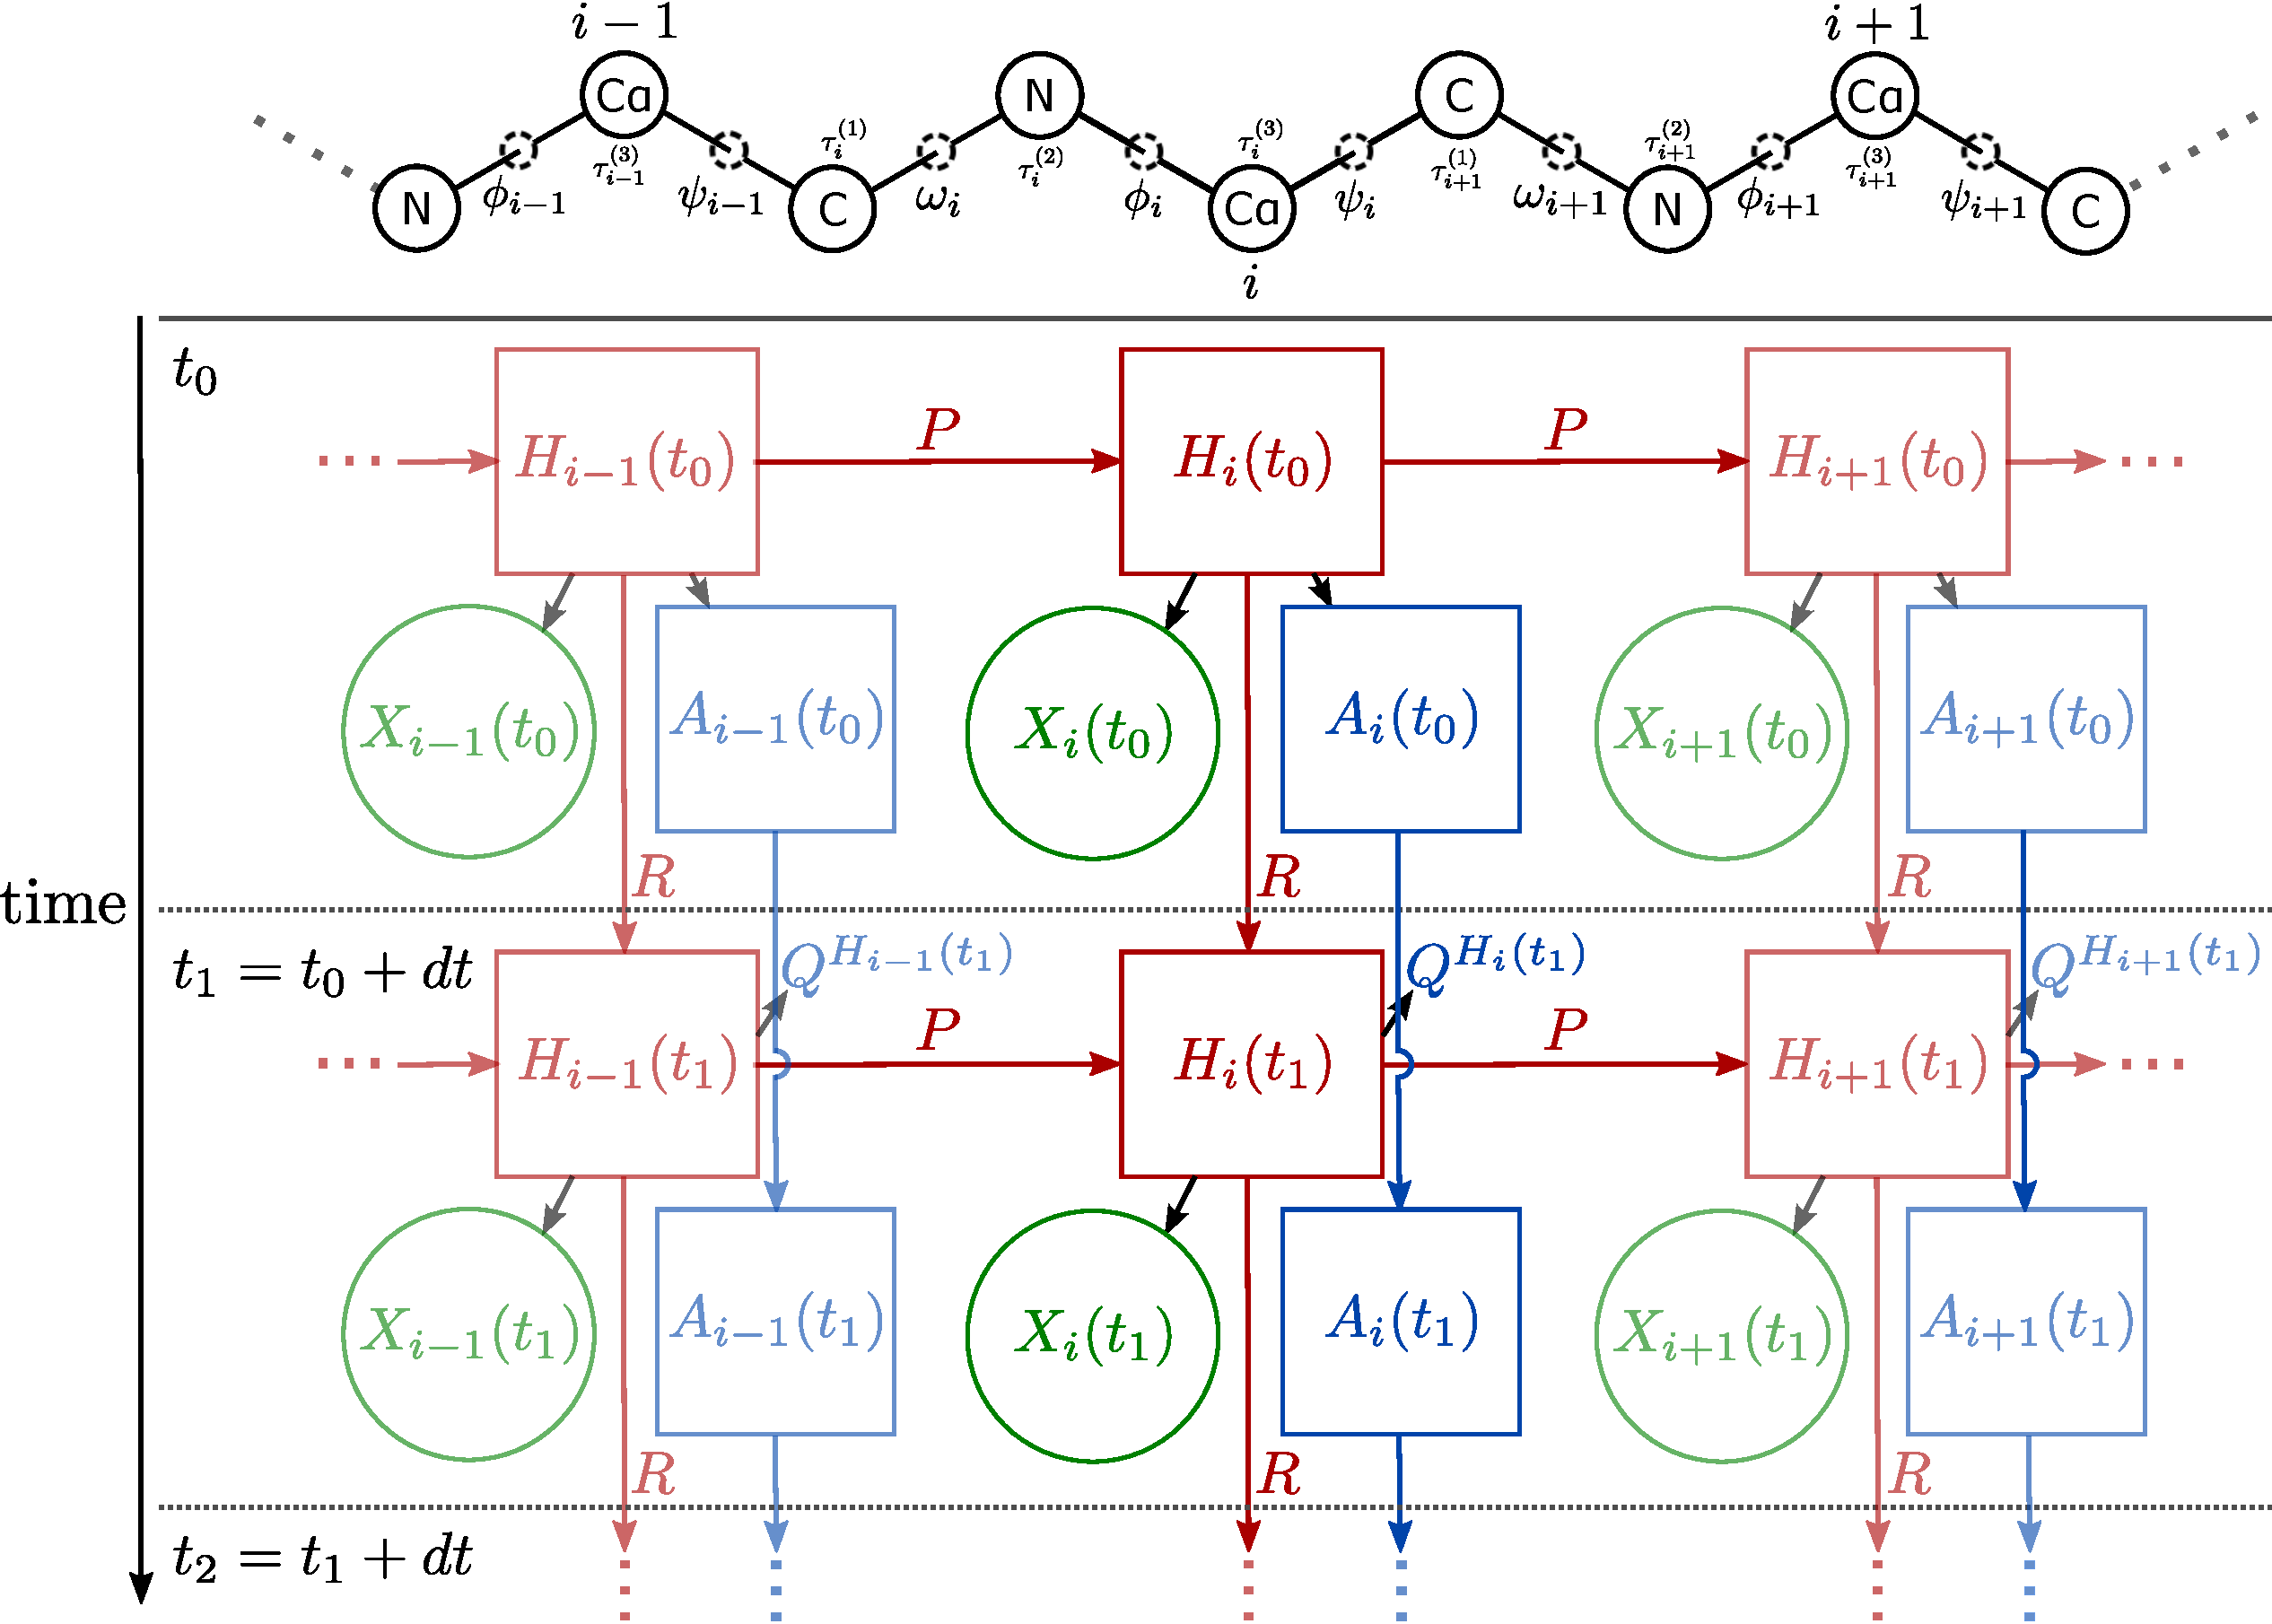
\includegraphics[width=2.0\columnwidth]{figures/model-structure-final.pdf}
	\caption{Graphical description of the model architecture.}%
	\label{fig:model-structure}%
\end{figure*}

\subsubsection{Hidden Markov model}
The hidden Markov model is given by: $\Pi$

\subsubsection{Rate matrix}
\begin{equation}
M_{ab}=\begin{cases}
\sqrt{\frac{\Pi(b)}{\Pi(a)}}Q_{a_{i}b_{i}}\pi^{h^{b}_{i}}_{aa^{b}_{i}} & \text{single amino acid difference at site $i$.}\\
\sqrt{\frac{\Pi(b)}{\Pi(a)}}R_{a_{i}b_{i}}\pi^{h^{b}_{i}}_{aa^{b}_{i}} & \text{single hidden state difference at site $i$.}\\
0 & \text{both hidden state and amino acid differences at site $i$.}\\
0 & \text{differences at two or more sites.}\\
-\underset{c\neq a}{\sum}M_{ac} & a=b
\end{cases}
\end{equation}

\subsubsection{Stationary distribution}
The stationary distribution is given by $p(a)$.

\section{Results}


\begin{table*}
	\captionsetup{justification=centering}
	\caption{\label{tab:sequencereconstruction} Ancestral sequence reconstruction benchmarks}	
	\begin{tabularx}{1.0\linewidth}{ccccc}
	\toprule
	Dataset & Our model & LG2008 & BEAST & ASR\\
	\midrule
	\rowcolor{black!20} Influenza & 0.896 & 0.876 & 0.88 & 0.87\tabularnewline
	HIV & 0.896 & 0.876 & 0.88 & 0.87\tabularnewline
	\bottomrule
	\end{tabularx}
\end{table*}

\section{Software availability}
Julia code (compatible with Windows and Linux) is available at: \href{https://github.com/michaelgoldendev/MESSI}{https://github.com/michaelgoldendev/MESSI}

\section{Acknowledgements}
MG is supported by the ERC under the European Union’s Seventh Framework Programme (FP7/2007-2013)/ERC grant agreement no. 614725-PATHPHYLODYN. 

\ifmbeformat
\section{Supplementary material}
Supplementary material is available  at Molecular Biology and Evolution
online: \url{http://www.mbe.oxfordjournals.org/}
\fi

\bibliographystyle{natbib}%%%%natbib.sty
\bibliography{refs}%%%refs.bib


\end{document}